\newpage

\section{Вычислительный эксперимент}

Для анализа моделей, полученных путем дистилляции модели учителя в модель ученика, проводится вычислительный эксперимент для задачи классификации.

Эксперимент проводится для выборок FashionMNIST~\cite{FMNIST} --- набора изображений предметов одежды и MNIST~\cite{MNIST} --- набора изображений рукописных цифр. В качестве модели учителя $\textbf{f}$ и модели ученика $\textbf{g}$ рассматривается многослойный перцептрон с четырьми и одним скрытыми слоями соответственно:

\begin{table}[h!t]
\begin{center}
\caption{Описание моделей}
\label{table_1}
\begin{tabular}{|c|c|c|}
\hline
	 & Учитель &\ Ученик\\
	\hline
	\multicolumn{1}{|l|}{Структура}
	& [784,256,128,64,64,10]& [784,64,10]\\
	\hline
	\multicolumn{1}{|l|}{Число параметров}
	& 246400 & 50816\\
\hline

\end{tabular}
\end{center}
\end{table}

Функция активации --- ReLu. Для решения оптимизационной задачи используется градиентный метод оптимизации Adam~\cite{Adam}.

Выборки разделяются на 4 части: обучающая, многоресурсная, малоресурсная, а также тестовая часть. Обучающая часть содержит 60000 объектов, многоресурсная часть содержит 59000 объектов, малоресурсная часть содержит 1000 объектов, а тестовая часть содержит 10000 объектов.

\begin{table}[h!t]
\begin{center}
\caption{Выборки}
\label{table_1}
\begin{tabular}{|c|c|c|}
\hline
	Выборка & Пояснение &\ Размер выборки\\
	\hline
	\multicolumn{1}{|l|}{FashionMNIST-Train}
	& Обучающая часть& 60000\\
	\hline
	\multicolumn{1}{|l|}{FashionMNIST-Big}
	& Многоресурсная часть& 59000\\
	\hline
	\multicolumn{1}{|l|}{FashionMNIST-Small}
	& Малоресурсная часть& 1000\\
	\hline
	\multicolumn{1}{|l|}{FashionMNIST-Test}
	& Тестовая часть& 10000\\
	\hline
	\multicolumn{1}{|l|}{MNIST-Train}
	& Обучающая часть& 60000\\
	\hline
	\multicolumn{1}{|l|}{MNIST-Big}
	& Многоресурсная часть& 59000\\
	\hline
	\multicolumn{1}{|l|}{MNIST-Small}
	& Малоресурсная часть& 1000\\
	\hline
	\multicolumn{1}{|l|}{MNIST-Test}
	& Тестовая часть& 10000\\
\hline

\end{tabular}
\end{center}
\end{table}

\newpage
\subsection{Анализ базовой дистилляции}

\paragraph{Обучение на всей выборке.}
Модели учителя и ученика обучаются на обучающей части FashionMNIST-Train.

\begin{figure}[h!t]\center
\subfloat[]
{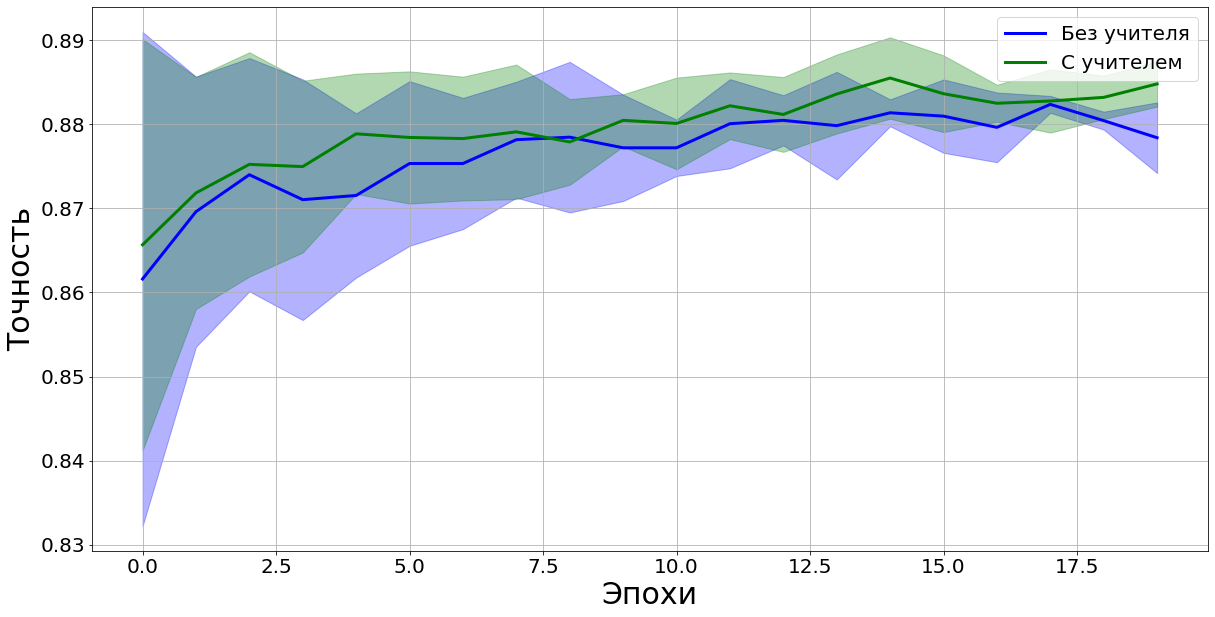
\includegraphics[width=0.5\textwidth]{results/acc}}
\subfloat[]
{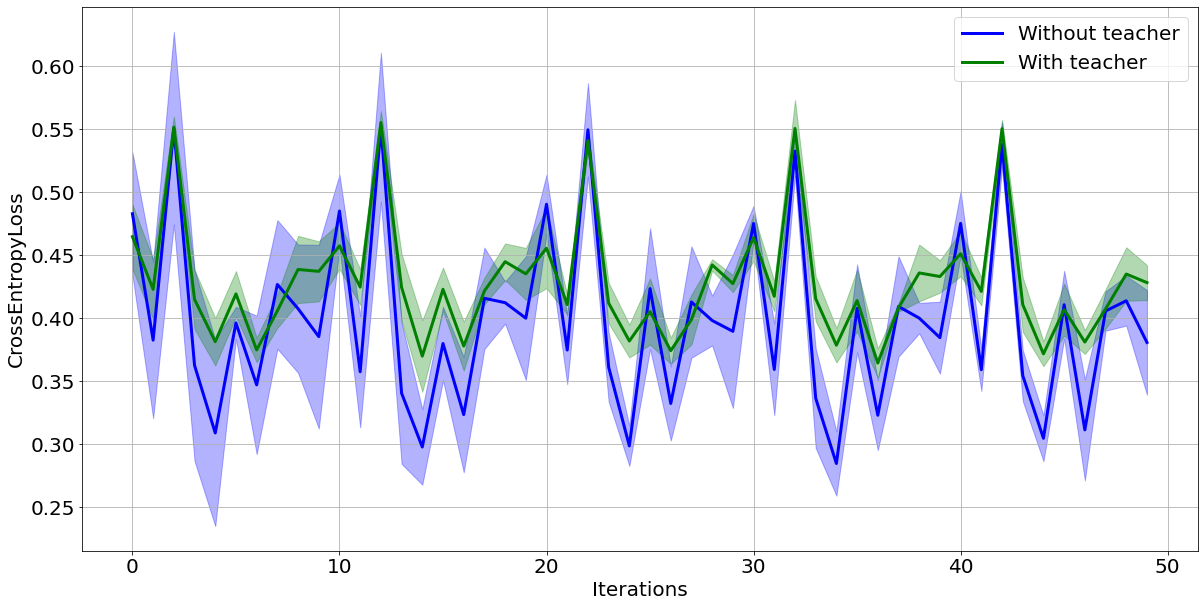
\includegraphics[width=0.5\textwidth]{results/loss}}\\
\caption{Качество аппроксимации на тестовой выборке. Все результаты усреднены по 5 запускам. a) точность; b) кросс-энтропийная ошибка между истинными и предсказанными учеником метками}
\end{figure}

На рис.1а показан график зависимости метрики точности на тестовой выборке между истинными метками объектов и вероятностями, предсказанными моделью ученика.

На рис.1б показан график зависимости кросс-энтропийной ошибки на тестовой выборке между истинными метками объектов и вероятностями, предсказанными моделью ученика.

На графиках видно, что модель, использующая метки учителя, показывает лучшее значение точности, при этом наблюдается значительное снижение кросс-энтропийной ошибки.

\newpage
\paragraph{Обучение на малоресурсной части.}
Модель учителя обучается на многоресурсной части FashionMNIST-Big, а модель ученика обучается на малоресурсной части FashionMNIST-Small.

\begin{figure}[h!t]\center
\subfloat[]
{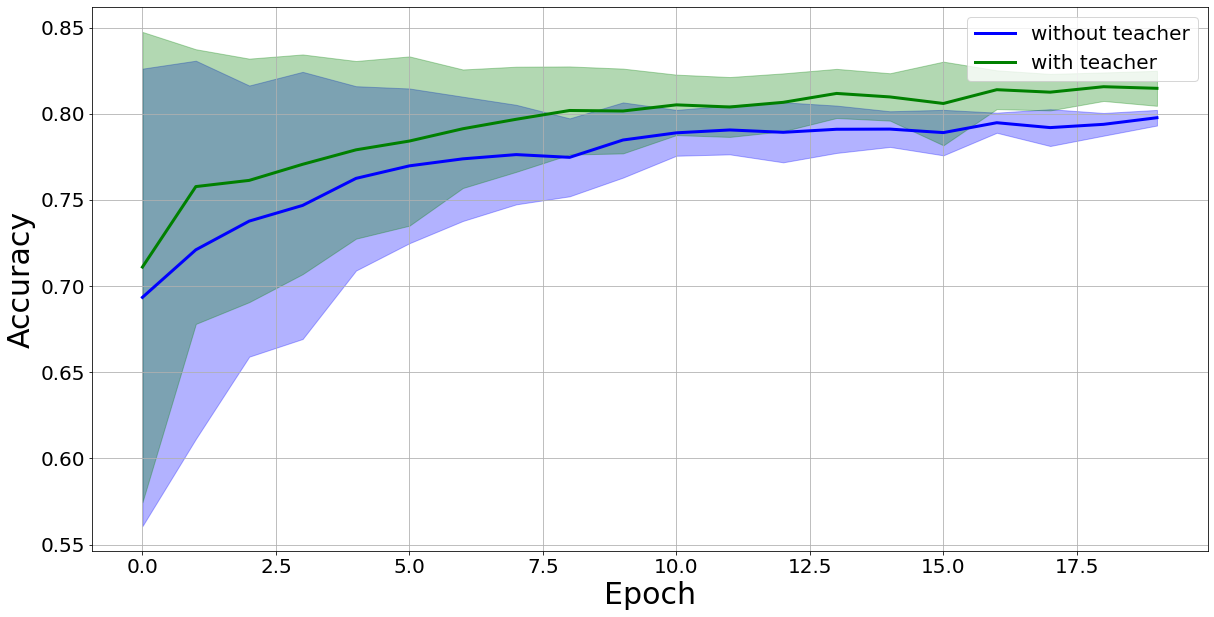
\includegraphics[width=0.5\textwidth]{results/small_acc}}
\subfloat[]
{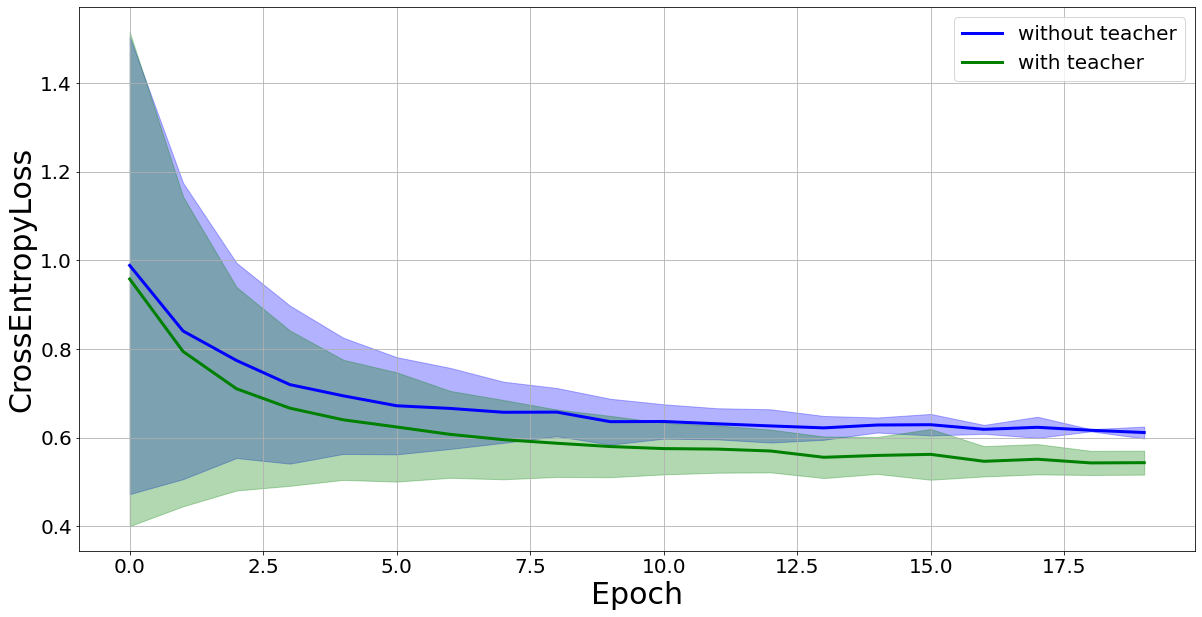
\includegraphics[width=0.5\textwidth]{results/small_loss}}\\
\caption{Качество аппроксимации на тестовой выборке. Все результаты усреднены по 5 запускам. a) точность; b) кросс-энтропийная ошибка между истинными и предсказанными учеником метками}
\end{figure}

На рис.2а показан график зависимости метрики  точности на тестовой выборке между истинными метками объектов и вероятностями, предсказанными моделью ученика.

На рис.2б показан график зависимости кросс-энтропийной ошибки на тестовой выборке между истинными метками объектов и вероятностями, предсказанными моделью ученика.

На графиках видно, что модель, использующая метки учителя, показывает лучшее значение точности, при этом наблюдается снижение кросс-энтропийной ошибки.

\newpage
\paragraph{Обучение на выборке с шумом.}
Добавим к многоресурсной части FashionMNIST-Big нормальный шум $\mathcal{N}\bigr(0,\frac{1}{10}\bigr)$ и обучим на нем модель учителя. Модель ученика обучается на малоресурсной части FashionMNIST-Small без шума.

\begin{figure}[h!t]\center
{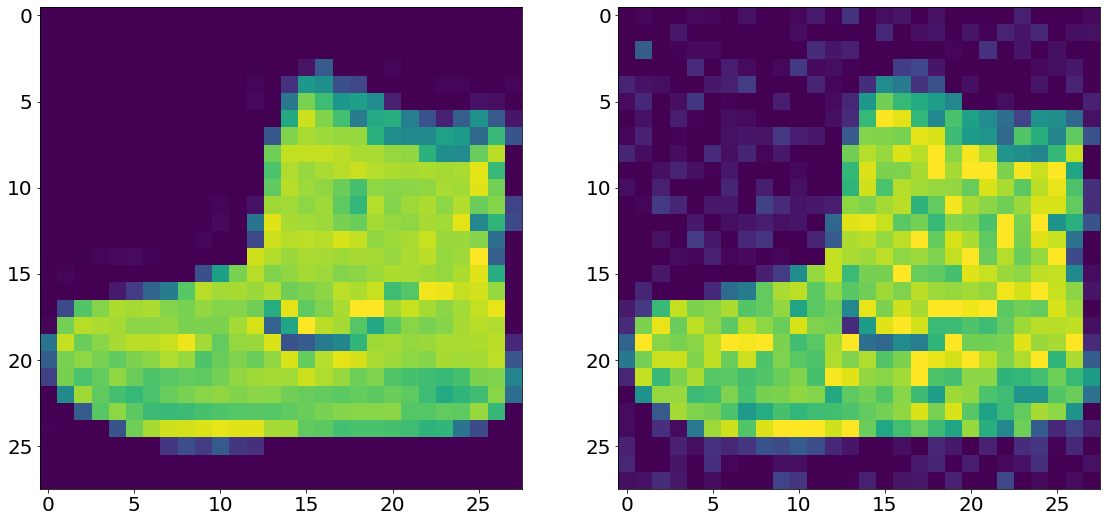
\includegraphics[width=0.5\textwidth]{results/noise}}
\caption{Сравнение объекта выборки до и после добавления шума}
\end{figure}\\

\begin{figure}[h!t]\center
\subfloat[]
{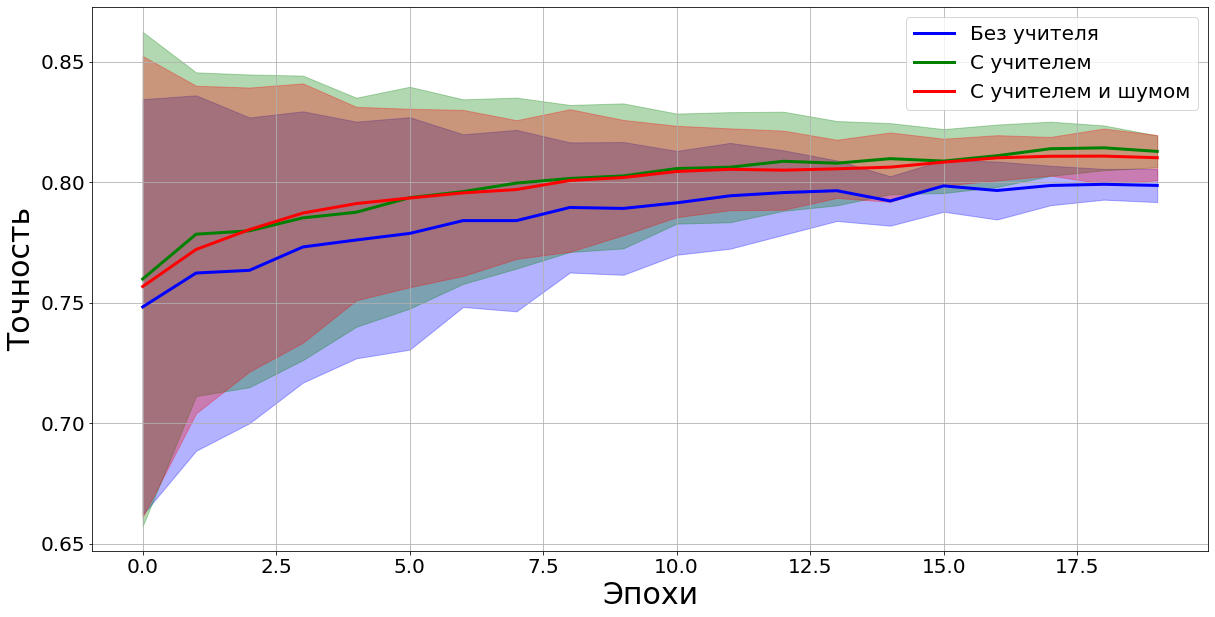
\includegraphics[width=0.5\textwidth]{results/noise_acc}}
\subfloat[]
{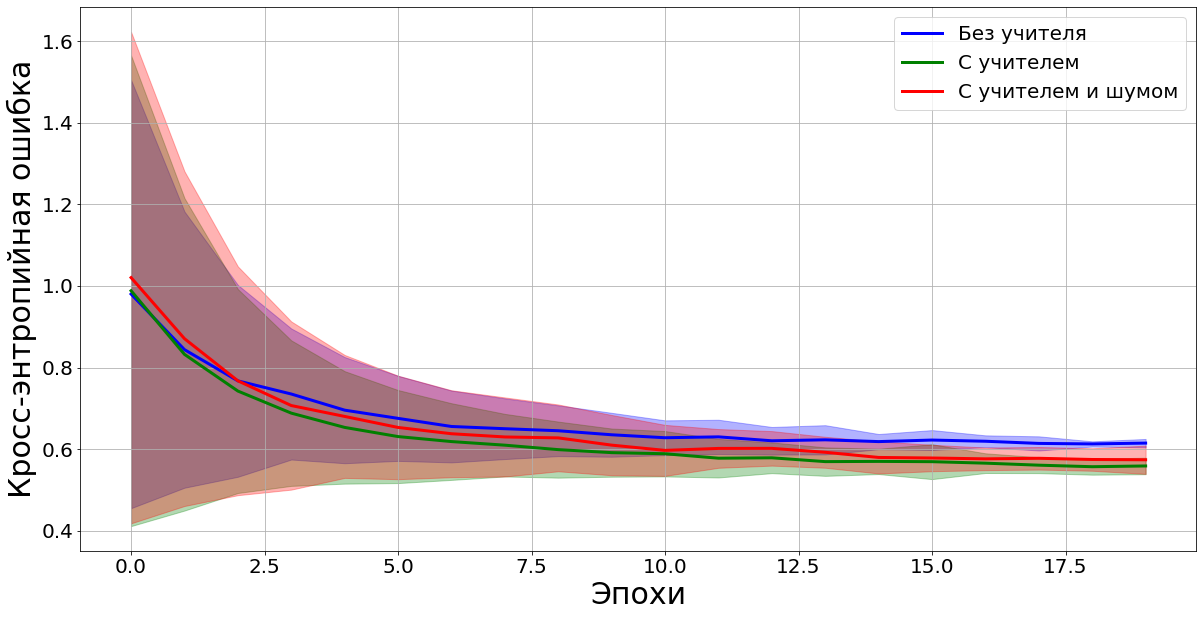
\includegraphics[width=0.5\textwidth]{results/noise_loss}}\\
\caption{Качество аппроксимации на тестовой выборке. Все результаты усреднены по 5 запускам. a) точность; b) кросс-энтропийная ошибка между истинными и предсказанными учеником метками}
\end{figure}

На рис.4а показан график зависимости метрики точности на тестовой выборке между истинными метками объектов и вероятностями, предсказанными моделью ученика.

На рис.4б показан график зависимости кросс-энтропийной ошибки на тестовой выборке между истинными метками объектов и вероятностями, предсказанными моделью ученика.

На графиках видно, что значения точности и кросс-энтропийной ошибки модели, использующей метки учителя на выборке с шумом, лежат между соответствующими значениями для модели без учителя и для модели, использующей метки учителя на выборке без шума.

Получаем, что шум в выборке не влияет на качество.

\paragraph{Обучение на выборке с dilation.}
Применим к многоресурсной части FashionMNIST-Big сверточное преобразование с параметром $\text{dilation}=2$ и обучим на нем модель учителя. Модель ученика обучается на малоресурсной части FashionMNIST-Small.

\begin{figure}[h!t]\center
{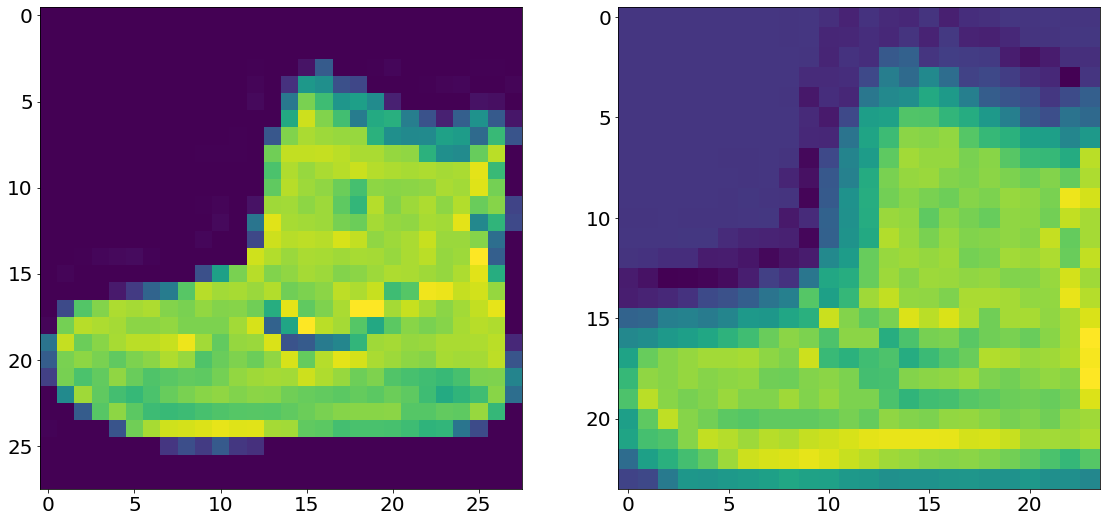
\includegraphics[width=0.5\textwidth]{results/dilation}}
\caption{Сравнение объекта выборки до и после преобразования}
\end{figure}\\

\begin{figure}[h!t]\center
\subfloat[]
{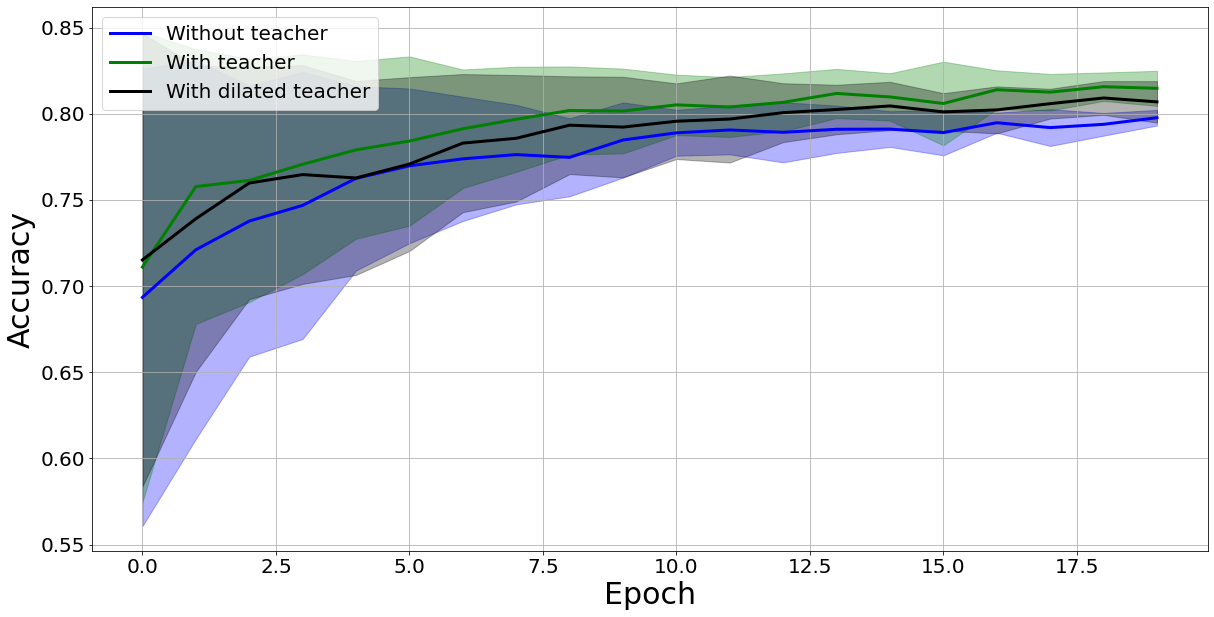
\includegraphics[width=0.5\textwidth]{results/dilation_acc}}
\subfloat[]
{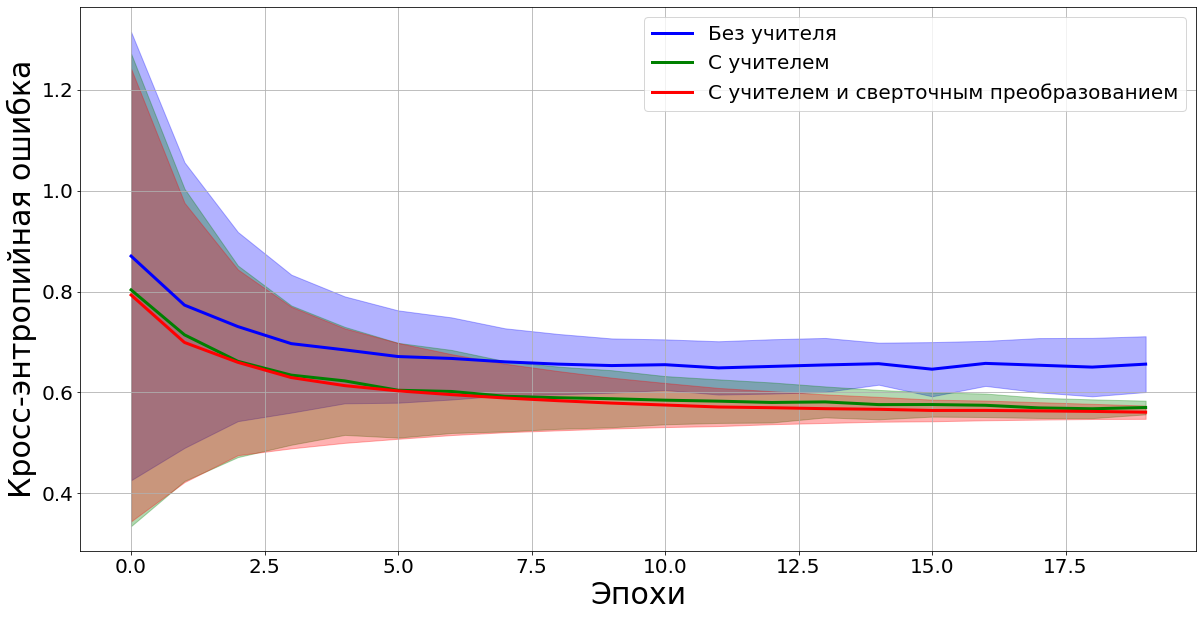
\includegraphics[width=0.5\textwidth]{results/dilation_loss}}\\
\caption{Качество аппроксимации на тестовой выборке. Все результаты усреднены по 5 запускам. a) точность; b) кросс-энтропийная ошибка между истинными и предсказанными учеником метками}
\end{figure}

На рис.6а показан график зависимости метрики точности на тестовой выборке между истинными метками объектов и вероятностями, предсказанными моделью ученика.

На рис.6б показан график зависимости кросс-энтропийной ошибки на тестовой выборке между истинными метками объектов и вероятностями, предсказанными моделью ученика.

На графиках видно, что значения точности и кросс-энтропийной ошибки модели, использующей метки учителя на выборке с преобразованием, лежат между соответствующими значениями для модели без учителя и для модели, использующей метки учителя на выборке без преобразования.

\subsection{Вариационный автокодировщик}

В качестве преобразования элементов выборки FashionMNIST~\cite{FMNIST} в элементы выборки MNIST~\cite{MNIST} используем модель вариационного автокодировщика~\cite{VAE}, аппроксимирующую отображение $\varphi$.
\paragraph{Базовая модель автокодировщика.} Данная модель состоит из двух частей. Сначала строится вероятностоное распределение в скрытом пространстве, которое позволяет генерировать скрытые представления для одного объекта. Далее с помощью декодировщика строится вероятностное распределение, позволяющее генерировать реконструкции исходного объекта.
\begin{enumerate}
    \item $q_{\alpha}(\mathbf{z}|\mathbf{x})$ --- вероятностный кодировщик;
    \item $p_{\beta}(\hat{\mathbf{x}}|\mathbf{z})$ --- вероятностный декодировщик;
    \item функция потерь:
    \[
    \begin{aligned}
    \mathcal{L}_{\text{VAE}}(\alpha, \beta)=\sum\limits_{i=1}^{l}\mathsf{E}_{\mathbf{z}\sim q_{\alpha}(\mathbf{z}|\mathbf{x}_{i})}\log{p_{\beta}(\mathbf{x}_{i}|\mathbf{z})} d \mathbf{z}-\mathsf{KL}(q_{\alpha}(\mathbf{z}|\mathbf{x}_{i}) || p(\mathbf{z})),
    \end{aligned}
    \]
    где
    $p(\mathbf{z})\sim \mathcal{N}(0,\sigma^{2}\mathbf{I})$ 
    --- априорное распределение.
\end{enumerate}
Получаем оптимизационную задачу:
$$\hat{\alpha}, \hat{\beta} = \arg\max_{\alpha, \beta} \mathcal{L}(\alpha, \beta).$$

\newpage
\paragraph{Генерация отображения из FashionMNIST в MNIST.}
Воспользуемся моделью вариационного автокодировщика~\cite{VAE} для преобразования изображений одежды из выборки FashionMNIST~\cite{FMNIST} в изображения цифр на основе выборки MNIST~\cite{MNIST}.

Создадим синтетическую выборку, где каждому изображению одежды выборки FashionMNIST-Train будет соответстовать случайное изображение цифры из выборки MNIST-Train из того же класса.

\begin{figure}[h!t]\center
\subfloat[]
{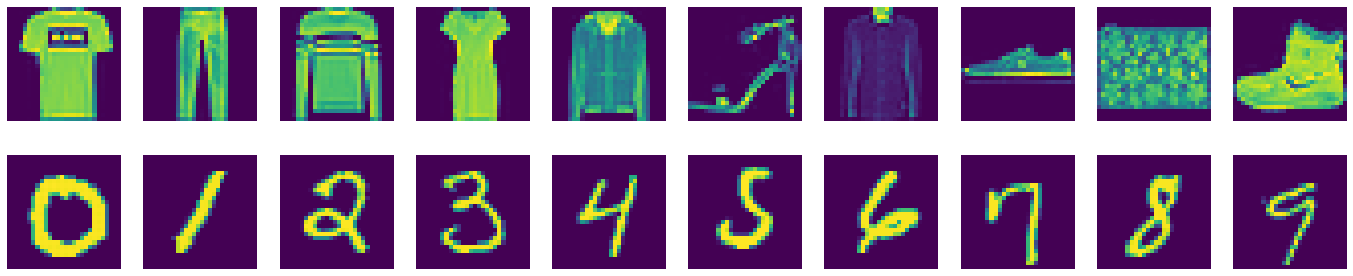
\includegraphics[width=0.8\textwidth]{results/fmnist_random_mnist_10.png}}
\qquad
\subfloat[]
{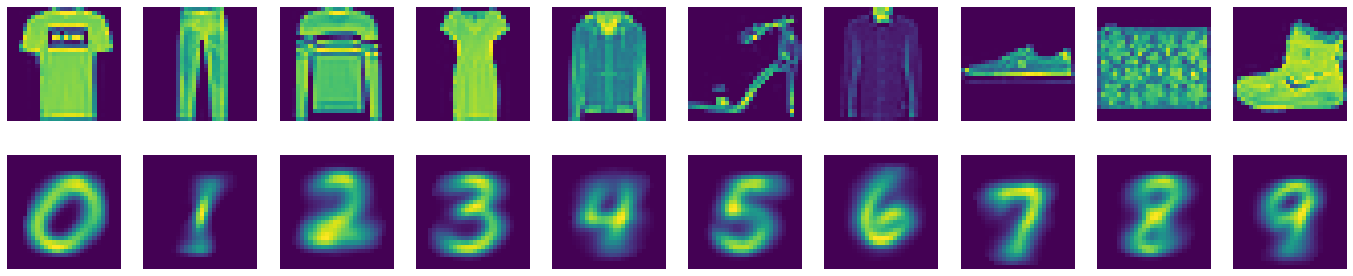
\includegraphics[width=0.8\textwidth]{results/fmnist_vae_mnist_10.png}}\\
\caption{a) Объекты синтетический выборки; b) Объекты исходной выборки до и после работы автокодировщика}
\end{figure}
Далее воспользуемся моделью вариационного автокодировщика~\cite{VAE}, состоящего из одного кодировщика и двух декодировщиков, соответствующих генерации объектов цифр и одежды соответственно. Используем модель с размером скрытого представления, равным 64.

\begin{figure}[h!t]\center
{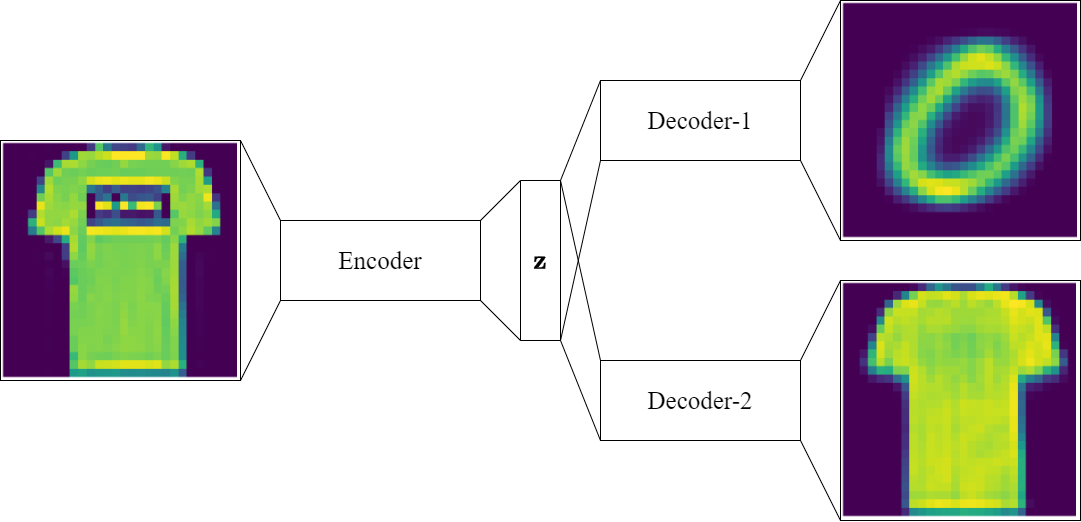
\includegraphics[width=0.8\textwidth]{results/VAE.png}}
\caption{Пример работы вариационного автокодировщика}
\end{figure}

На основе полученной выборки обучим модель вариационного автокодировщика~\cite{VAE}, минимизируя ошибку между выходом модели и исходным значением --- изображением одежды и ошибку между выходом модели и целевым значением --- изображением цифр, соответствующего исходному объекту.

Полученная модель генеририрует семейство новых объектов --- изображений цифры и изображений одежды для одного и того же изображения одежды.

\newpage

Проанализируем изменение выхода модели при изменении случайного вектора в скрытом представлении. Для визуализации рассмотрим скрытое представление размерности 2:

\begin{figure}[h!t]\center
\subfloat[]
{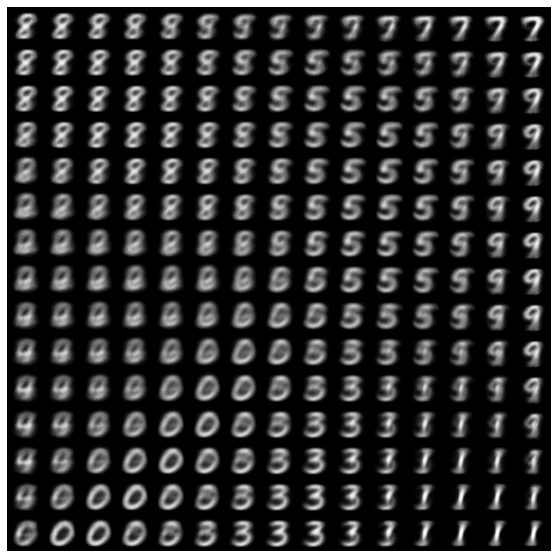
\includegraphics[width=0.4\textwidth]{results/decoder_digits.png}}
\qquad
\subfloat[]
{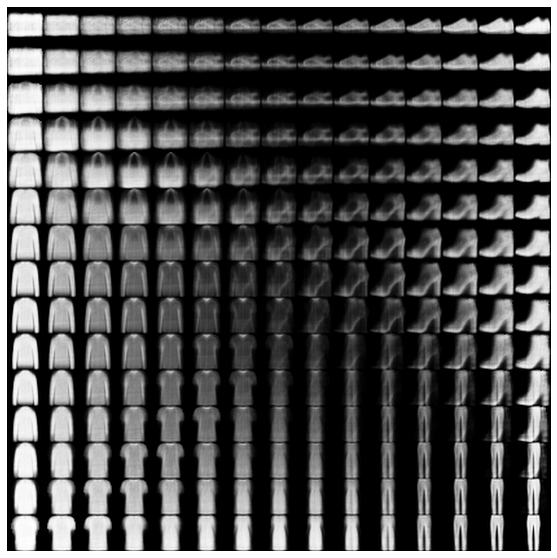
\includegraphics[width=0.4\textwidth]{results/decoder_fashion.png}}\\
\caption{Зависимость выхода модели от изменения вектора в скрытом представлении для генерации a) цифр; b) одежды}
\end{figure}

Видно, что классы соответствуют друг другу, как представлено на рис.7а. То есть рис.9 не противоречит рис.7.

\subsection{Анализ качества модели, предложенной на основе вариационного автокодировщика}

Обучается модель учителя на выборке MNIST-Big, а модель ученика на выборке FashionMNIST-Small. При этом при обучении модели ученика будем использовать метки учителя, подавая ему на вход выход вариационного автокодировщика~\cite{VAE}, переводящего изображения одежды в изображения цифр.

Сравнивается качество аппроксимации без использования вариационного автокодировщика~\cite{VAE}: модель ученика обучается на выборке FashionMNIST-Small, модель учителя обучается на выборке MNIST-Big и используется при обучении ученика, получая на вход изображения одежды без преобразования вариационным автокодировщиом.\\

\begin{figure}[h!t]\center
\subfloat[]
{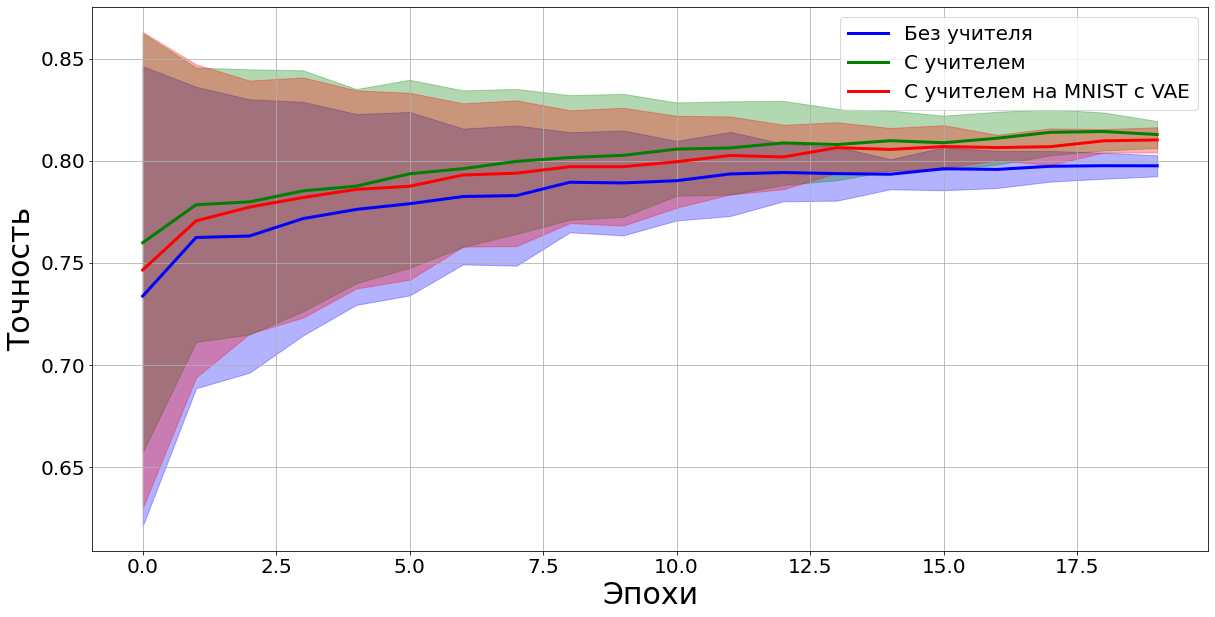
\includegraphics[width=0.5\textwidth]{results/vae_acc}}
\subfloat[]
{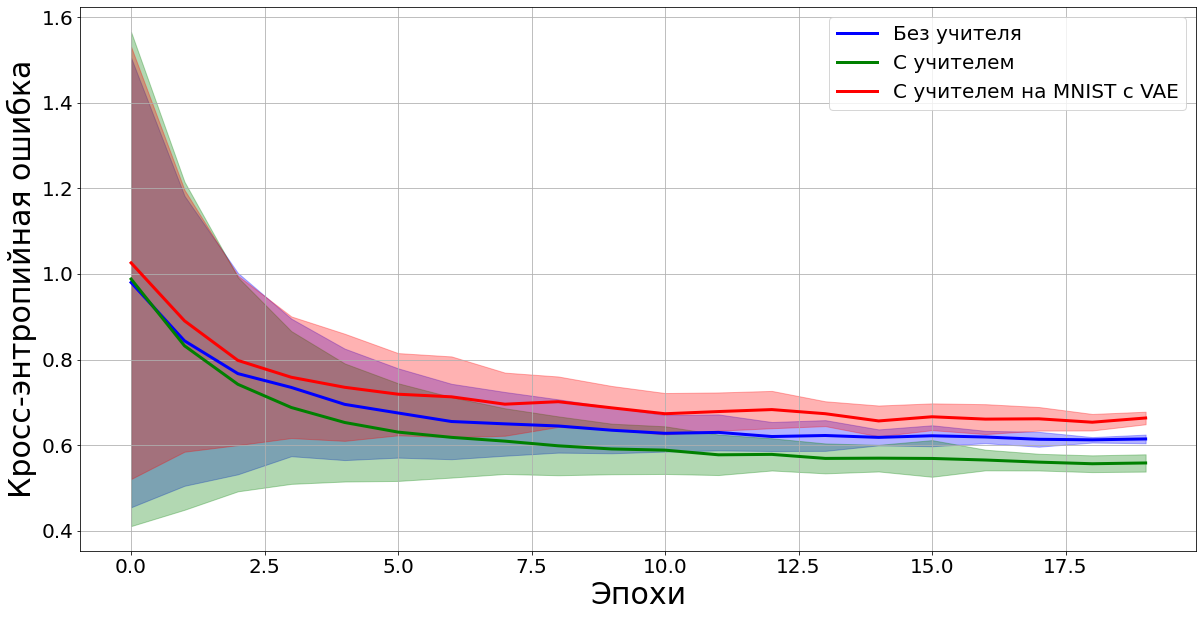
\includegraphics[width=0.5\textwidth]{results/vae_loss}}\\
\caption{Качество аппроксимации при использовании VAE на малодоменной выборке. Все результаты усреднены по 5 запускам. a) точность; b) кросс-энтропийная ошибка между истинными и предсказанными учеником метками}
\end{figure}\\

\begin{figure}[h!t]\center
\subfloat[]
{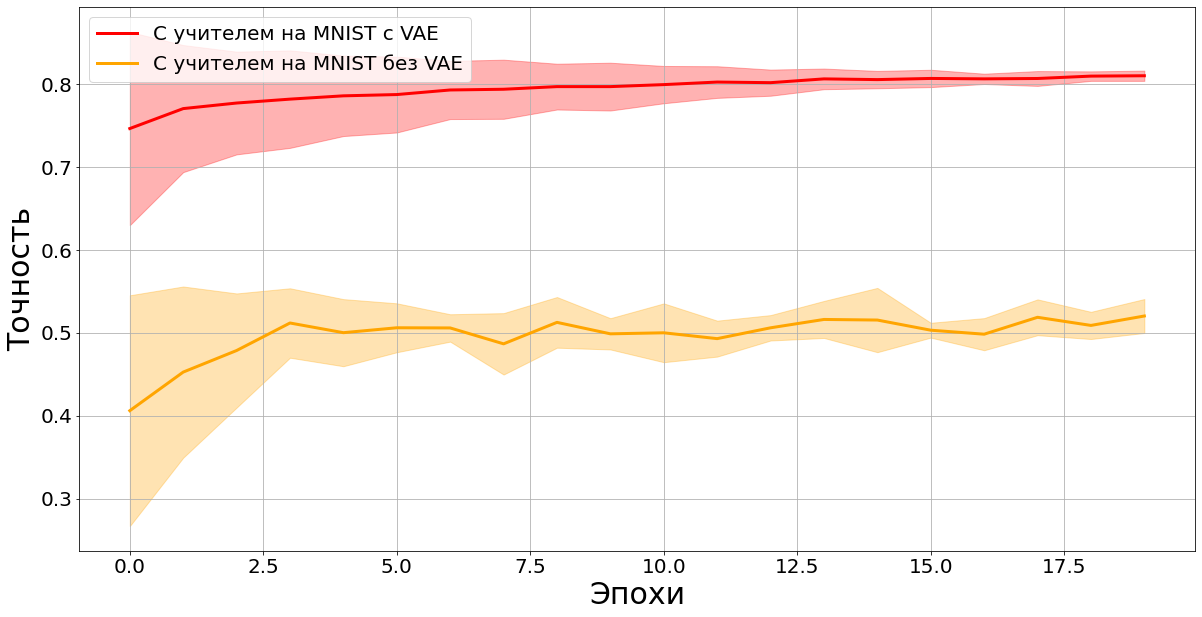
\includegraphics[width=0.5\textwidth]{results/vae_acc_comparison}}
\subfloat[]
{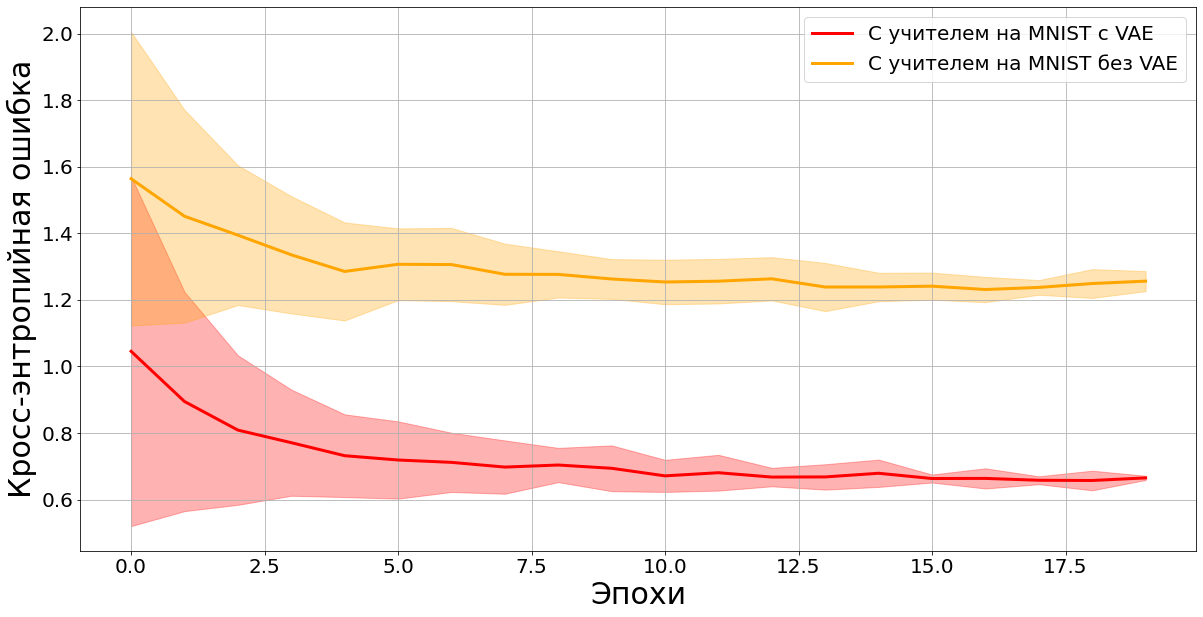
\includegraphics[width=0.5\textwidth]{results/vae_loss_comparison}}\\
\caption{Сравнение качества аппроксимации в зависимости от использования VAE на малодоменной выборке. Все результаты усреднены по 5 запускам. a) точность; b) кросс-энтропийная ошибка между истинными и предсказанными учеником метками}
\end{figure}

На графиках видно, что без использования отображения $\varphi$ модель становится более шумной с явным понижением качества аппроксимации.

\newpage
\subsection{Анализ качества модели на расширенной синтетически сгенерированной выборке}
На основе малоресурсной части выборки FashionMNIST-Small сформируем новую выборку, сгенерировав для каждого объекта одежды 70 изображений цифр с помощью модели вариационного автокодировщика~\cite{VAE}. Далее разделим полученную выборку на 4 части: обучающая, многоресурсная, малоресурсная, а также тестовая часть. Обучающая часть содержит 60000 объектов, многоресурсная часть содержит 59000 объектов, малоресурсная часть содержит 1000 объектов, а тестовая часть содержит 10000 объектов.
\begin{table}[h!t]
\begin{center}
\caption{Расширенная сгенерированная выборка}
\label{table_1}
\begin{tabular}{|c|c|c|}
\hline
	Выборка & Пояснение &\ Размер выборки\\
	\hline
	\multicolumn{1}{|l|}{GeneratedMNIST-Train}
	& Обучающая часть& 60000\\
	\hline
	\multicolumn{1}{|l|}{GeneratedMNIST-Big}
	& Многоресурсная часть& 59000\\
	\hline
	\multicolumn{1}{|l|}{GeneratedMNIST-Small}
	& Малоресурсная часть& 1000\\
	\hline
	\multicolumn{1}{|l|}{GeneratedMNIST-Test}
	& Тестовая часть& 10000\\

\hline

\end{tabular}
\end{center}
\end{table}

Модель ученика обучается на малоресурсной части FashionMNIST-Small, модель учителя на многоресурсной части GeneratedMNIST-Big сгенерированной расширенной выборки и используется при обучении ученика.

\begin{figure}[h!t]\center
\subfloat[]
{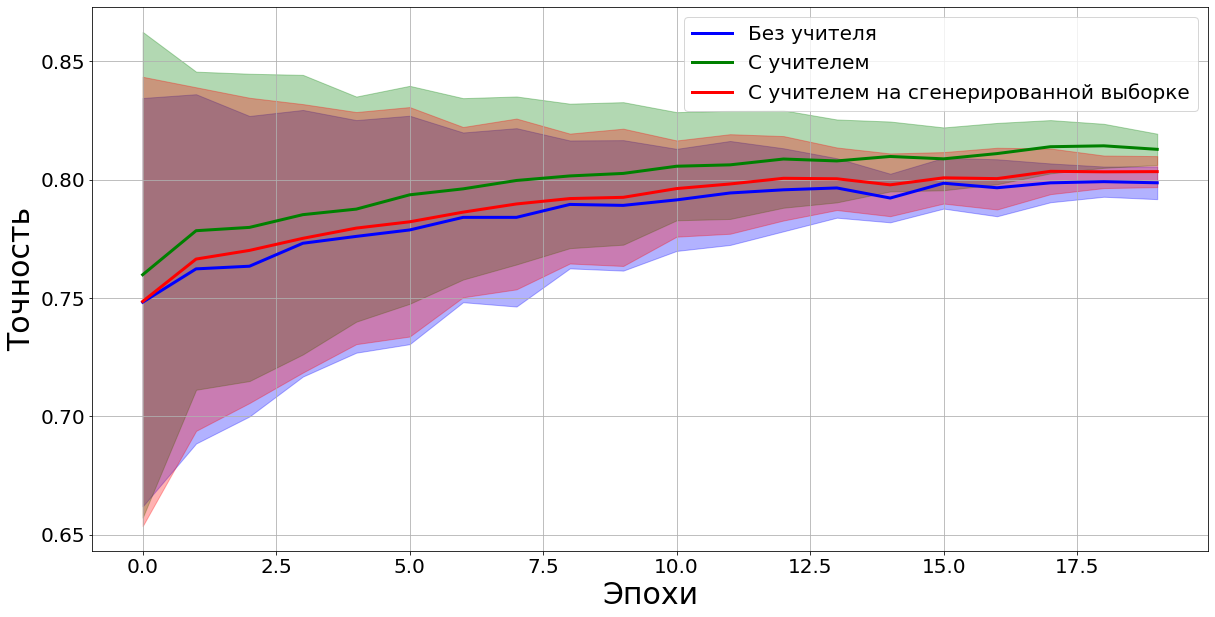
\includegraphics[width=0.5\textwidth]{results/ext_mnist_acc.png}}
\subfloat[]
{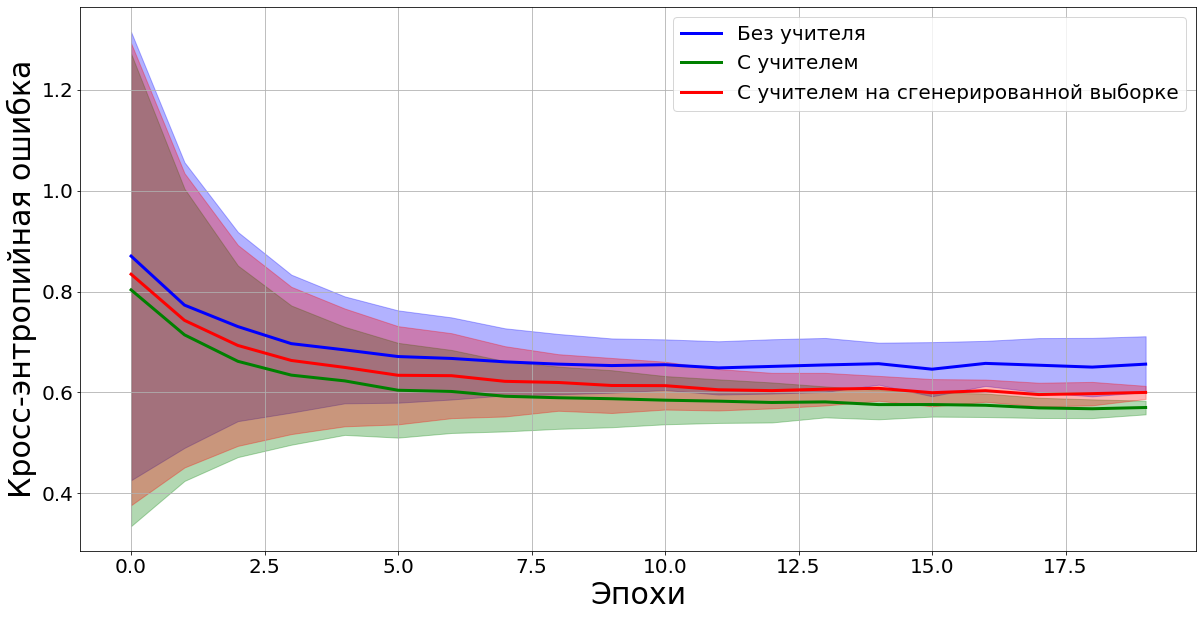
\includegraphics[width=0.5\textwidth]{results/ext_mnist_loss.png}}\\
\caption{Качество аппроксимации на тестовой выборке. Все результаты усреднены по 5 запускам. a) точность; b) кросс-энтропийная ошибка между истинными и предсказанными учеником метками}
\end{figure}\\

На графиках видно, что значения точности и кросс-энтропийной ошибки модели, использующей метки учителя, обученного на сгенерированной расширенной выборке, лежат между соответствующими значениями для модели без учителя и для модели, использующей метки учителя, обученного на многоресурсной части выборки.